\documentclass[12pt,a4paper]{article}
\usepackage{datetime}
\usepackage{hyperref}
\usepackage{graphicx}
\usepackage{color}
\usepackage{amsmath}

\begin{document}

\title{BOLODSP Software User's Guide}

\author{Jack Lovell\thanks{\url{jack.lovell@durham.ac.uk}}}

\date{\today}

\maketitle

\abstract
This document serves as a guide for the end user to work with the BOLODSP software package which is bundled with D-TACQ's ACQ400 series firmware. A basic theory of operation is presented, and the parameters which control the operation of the BOLODSP module are discussed. General operation of D-TACQ's software, and the implementation details of the software and associated FPGA firmware module, are out of scope.

\tableofcontents

\section{Introduction}
The BOLODSP software package is part of a custom module for D-TACQ ACQ400 series products used to operate the BOLO8BLF hardware module. It provides software control of the BOLODSP FPGA module through a series of Linux commands, as well as some helper applications to simplify the fine tuning of the signal processing capabilities of the module.

This document is \textit{not} a general user guide for D-TACQ software. For that, refer to the D-TACQ 4G user guide at \url{http://www.d-tacq.com}. It is only concerned with the commands and settings provided by the package itself. Likewise, any requests for support with operating a system with this package installed should be directed to D-TACQ directly, and not to the author, unless the query is specifically about an aspect of the BOLODSP module.

\section{Theory of Operation}
\subsection{Voltage Measurement}
\begin{figure}
  \centering
  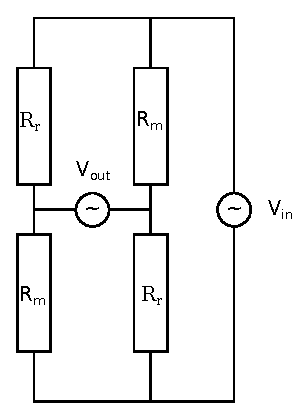
\includegraphics[width=0.3\textwidth]{sensor_schematic.eps}
  \caption{Electrical schematic of bolometer sensor}
  \label{fig:sensor}
\end{figure}
A resistive bolometer consists of 4 resistors in a Wheatstone bridge configuration (see Figure~\ref{fig:sensor}). The two resistors marked $R_m$ are ``measurement'' resistors, which are in thermal contact with a thin foil. Incident radiation heats the foil and hence the resistors, increasing their resistance. The two resistors marked $R_r$ are ``reference'' resistors: they are not in contact with the foil, and so their temperature (and hence resistance) remain constant.

When a voltage $V_{in}$ is applied across one diagnoal of the bridge as shown, there will be zero output voltage $V_{out}$ if the bridge is balanced. However, if the measurement resistors have increased resistance compared to the reference resistors, the bridge will be unbalanced, and $V_{out}$ will be non-zero. By measuring $V_{out}$ it is therefore possible to calculate the resistance change of the foil, and by knowing the electrical and thermal properties of the sensor it is possible to then infer the temperature change and the absorbed power. The details of these calculations are out of the scope of this document.

To minimise noise in the system, AC synchronous detection is used to measure $V_{out}$. An AC excitation voltage $V_{in}$ is applied to the bridge, typically a sinusoid with a frequency of a few 10s of kHz. The amplitude of $V_{out}$ at the same frequency is measured, and this voltage amplitude is used in the bolometer equation to determine the absorbed power. The amplitude calculation (demodulation) is performed on the FPGA module, as follows.

The excitation voltage $V_{in}$ is of the form
\begin{equation}
  \label{equ:vin}
  V_{in} = V_0\sin(\omega t)
\end{equation}
Where $V_0$ is the amplitude of the excitation voltage and $\omega$ is the frequency. The output from the bridge due to the bridge imbalance is of the form:
\begin{equation}
  \label{equ:vout}
  V_{out} = A\sin(\omega t + \phi)
\end{equation}
Where the amplitude $A$ is the quantity we want to measure, and $\phi$ is the phase difference between the output and excitation voltages. This phase shift is due to round trip time and parasitic capacitance in the system, and can be significant when there is a long cable between the electronics and the sensor.

By multiplying $V_{out}$ with a normalised form of $V_{in}$ (which we shall call $V_{ref,i}$) and time averaging to remove the $2\omega$ frequency component from the resulting signal, we can obtain the amplitude, assuming it varies slowly compared to the time averaging window. This is known as the ``in-phase'' component, since the signal is multiplied by a reference voltage of the same phase as the excitation voltage:
\begin{equation}
  \label{equ:I}
  \begin{split}
  I &= \frac{1}{n\pi}\int_{0}^{2n\pi}V_{ref,i}V_{out}\mathrm{d}\omega t \\
  &= \frac{1}{n\pi}\int_{0}^{2n\pi}\sin(\omega t) A \sin(\omega t + \phi)\mathrm{d}\omega t \\
  &= \frac{A}{2}\cos \phi
  \end{split}
\end{equation}
Equation~\ref{equ:I} still depends on the phase $\phi$. Traditionally, some phase shift has been applied to $V_{ref,i}$ such that $\phi = 0$ to remove the phase dependence on $I$, but we employ a more general method. Consider a second reference, $V{ref,q}$ which is a quarter of a period out of phase with the excitation voltage:
\begin{equation}
  \label{equ:Q}
  \begin{split}
  Q &= \frac{1}{n\pi}\int_{0}^{2n\pi}V_{ref,q}V_{out}\mathrm{d}\omega t \\
  &= \frac{1}{n\pi}\int_{0}^{2n\pi}\cos(\omega t) A \sin(\omega t + \phi)\mathrm{d}\omega t \\
  &= -\frac{A}{2}\sin \phi
  \end{split}
\end{equation}
We can now combine Equations~\ref{equ:I} and~\ref{equ:Q} to remove the phase dependence:
\begin{equation}
  \label{equ:A}
  A = 2\sqrt{I^2 + Q^2}
\end{equation}
Equation~\ref{equ:A} thus gives a measure of the amplitude of the output voltage independent of phase, and hence independent of the hardware used. This method is known as ``quadrature detection''.

For completeness, the phase is given by:
\begin{equation}
  \label{equ:phi}
  \phi = -\tan^{-1}\left(\frac{Q}{I}\right)
\end{equation}

\subsection{Voltage Offset}
No sensor is perfect, in the sense that the bridge will never be perfectly balanced in the absense of any input power. Likewise, no electronics is perfect, and there will always be some cross talk between excitation and measurement voltages. This leads to a voltage offset with no input power:
\begin{equation}
  \label{equ:voff}
  V_{off} = A_{off}e^{i\phi_{off}}
\end{equation}
Note that the offset voltage has both an amplitude \textit{and} phase, which may be different to the phase of the signal due to incident power, making the measured voltage a complex signal. It is necessary to subtract this offset from the measured signal using a suitable complex subtraction, either by decomposing into real ($I$) and imaginary ($Q$) parts and subtracting the real and imaginary parts respectively of the offset, or by performing a vector-based subtraction using the cosine rule.

The FPGA firmware has the capability to perform the first of these methods on-chip, using user-loadable offset values for each channel. When offset subtraction has been correctly performed, the remaining phase should be constant (being only a property of the geometry), and the remaining amplitude will be a measure only of the bridge imbalance (and hence the temperature change of the sensor foil). The phase is therefore a useful measurement for data validation.

\end{document}
